
%%%%%%%%%%%%%%%%%%%%%%%%%%%%%%%%%%%%%%%%%%%%%%%%%%%%%%%%%%%%%%%%%%%%%%%%%%%%%%
%%% Preamble

%%% Document Type
\documentclass[11pt]{article}

%%% Packages
\usepackage{amsmath,amssymb,cancel,units} % math environment and symbols
\usepackage{array}                        % for better arrays (eg matrices) in maths
\usepackage{paralist}                     % very flexible & customisable lists (eg. enumerate/itemize, etc.)
\usepackage{verbatim}                     % adds environment for commenting out blocks of text & for better verbatim
\usepackage[pdftex,bookmarks,colorlinks,breaklinks]{hyperref}  % PDF hyperlinks, with coloured links
\usepackage{memhfixc}                     % remove conflict between the memoir class & hyperref
\usepackage{graphicx}                     % Add graphics capabilities
\usepackage{xspace}                        % smart space insertion after commands
\usepackage{tabulary}
\usepackage{listings}
\usepackage[table]{xcolor} % http://tex.stackexchange.com/questions/5363/how-to-create-alternating-rows-in-a-table

%%% Notation and Variables

\newcommand{\targetData}{D}
\newcommand{\trainingDataForModel}[1]{D^{*#1}}
\newcommand{\trainingDataSet}{\mathbf{D}^{*}}
\newcommand{\summaryStatisticFunction}{S}
\newcommand{\modelCategory}[1]{M_{#1}}
\newcommand{\modelCategories}{\mathbf{M}}

%%%%%%%%%%%%%%%%%%%%%%%%%%%%%%%%%%%%%%%%%%%%%%%%%%%%%%%%%%%%%%%%%%%%%%%%%%%%%%%
%% Main Document
\begin{document}
% \rowcolors{2}{gray!25}{gray!15}

\title{ARCHIPELAGO}
\author{Jeet Sukumaran}
\maketitle

\section{Introduction}

``Archipelago'' is the name of a generative phylogeny-based model that simultaneously incorporates the diversification processes of speciation and extinction nad the biogeographical processes of area gain (``dispersal'') and area loss (``extirpation''), with these processes being differentially regulated by ecological or other traits that are themselves co-evolving on the phylogeny.
The theory and background to this model and its usage is described in the following paper:


This software project, ``archipelago'' presents a suite of programs to generate and analyze data under the Archipelago model.
The primary objective of the analysis is \textit{model selection}: i.e., statistically identifying the model that generated a particular set of data.
% to \textit{classify a dataset with respect to the model that generated it}.
``archipelago'' is, thus, a computational biogeographical model selection analysis package that exploits the power and flexibility of the Archipelago model to allow you to ask and answer historical biogeographical questions of a nature and complexity that are not possible under any other approach.
In particular, instead of asking questions about ancestral area patterns, you can ask questions about processes, and how some processes (e.g., ecology) affect other processes (e.g., dispersal or speciation).

As an example of a very basic analysis, let us consider testing whether or not dispersal is constrained by habitat association of a lineage (Figure).
\begin{figure}[h!]
    \begin{center}
        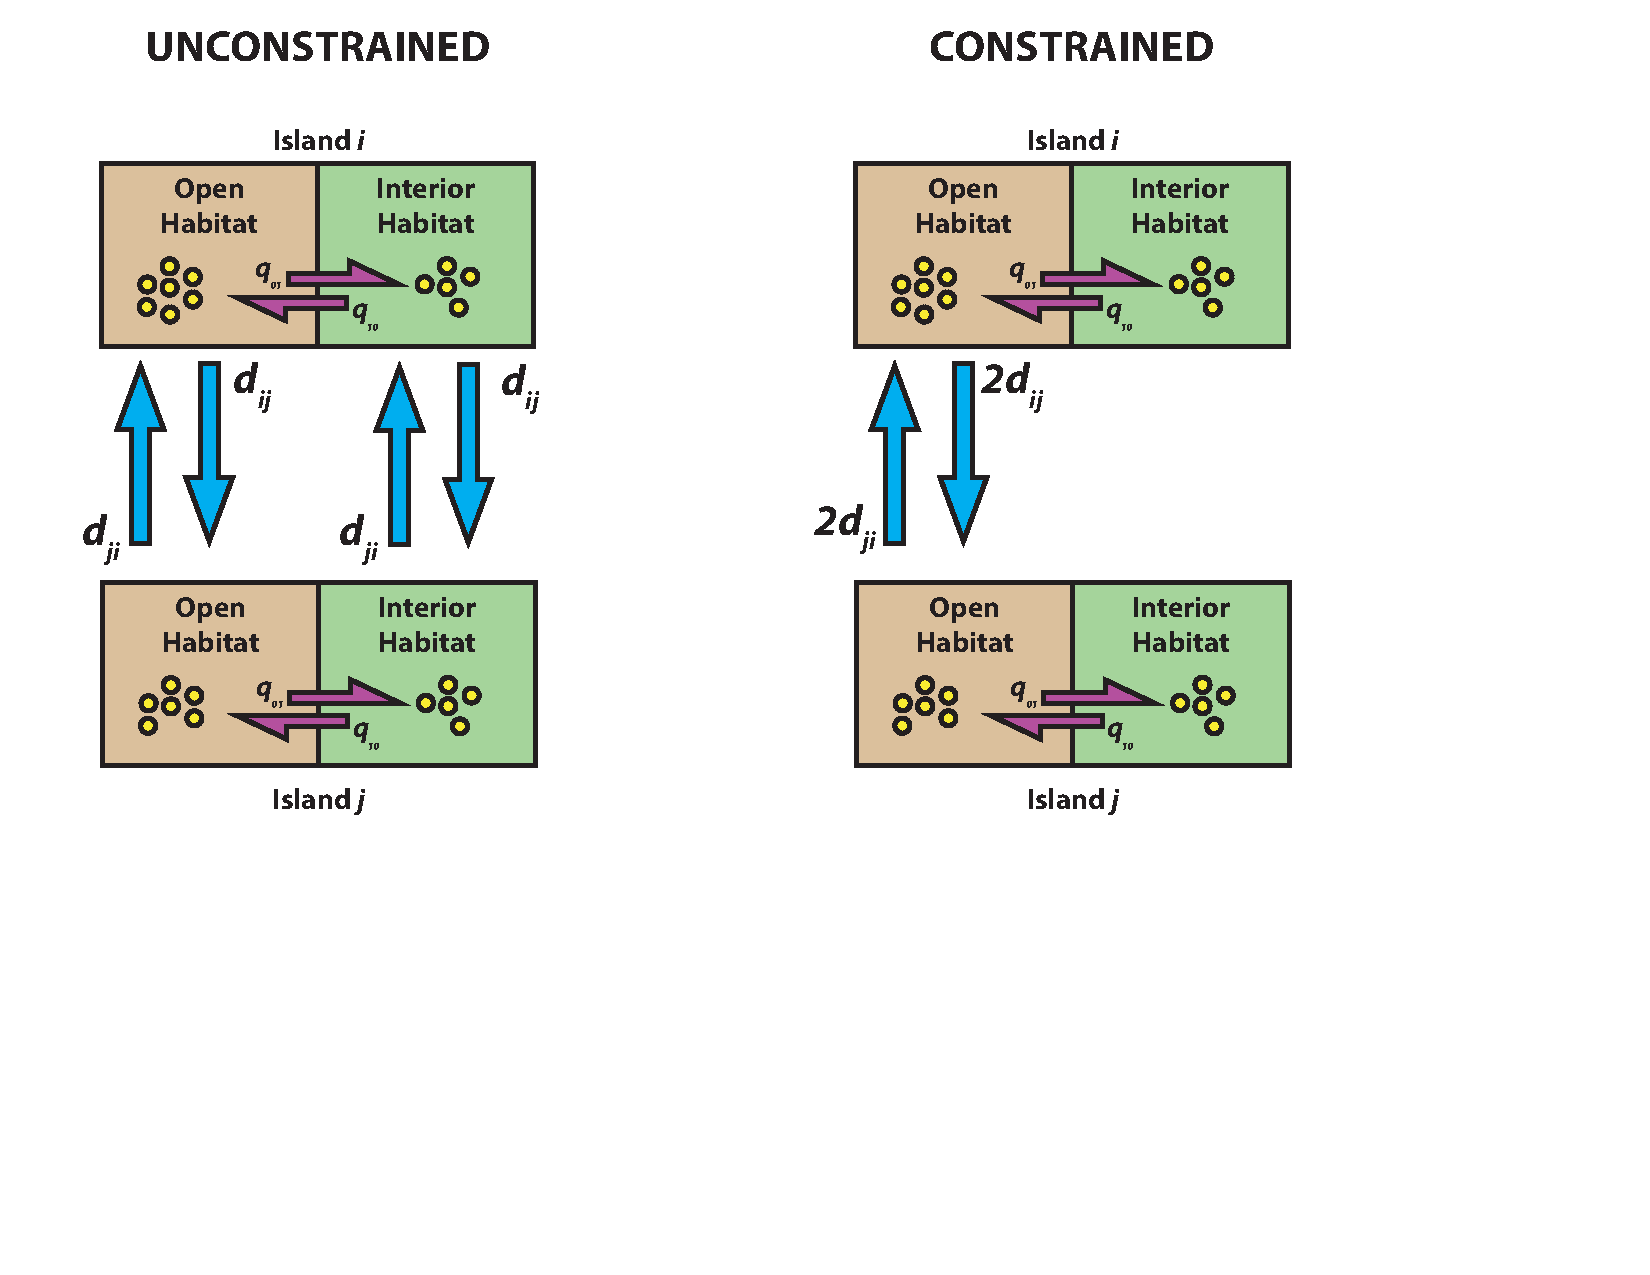
\includegraphics[scale=0.5]{figs/Experimental-Design-1.pdf}
        % \caption{default}
        % \label{fig:default}
    \end{center}
\end{figure}
We propose two different models, each corresponding to a different dispersal regime.
In the ``unconstrained'' model, lineages are free to disperse between islands regardless of their habitat affinities.
In the ``constrained'' model, ony lineages associated with the disturbed or open habitats can disperse between islands, while lineages associated with interior habitats are not able to disperse.

\section{Installation}

\subsection{Pre-requisites}

\begin{itemize}
    \item Python 2.7 or higher
    \item DendroPy Phylogenetic Computing Library, version 4 or above (\url{http://dendropy.org}).
    \item R (\url{http://www.r-project.org/})
    \item The following R packages:
    \begin{itemize}
        \item adegenet
        \item picante
        \item BioGeoBears
        \item GEIGER
    \end{itemize}
\end{itemize}

\subsection{Installation from Source}

Run the following in the top-level directory of the project:

\begin{lstlisting}
    python setup.py install
\end{lstlisting}


\section{Usage}

\subsection{Overview of Workflow}

\begin{figure}[h!]
    \begin{center}
        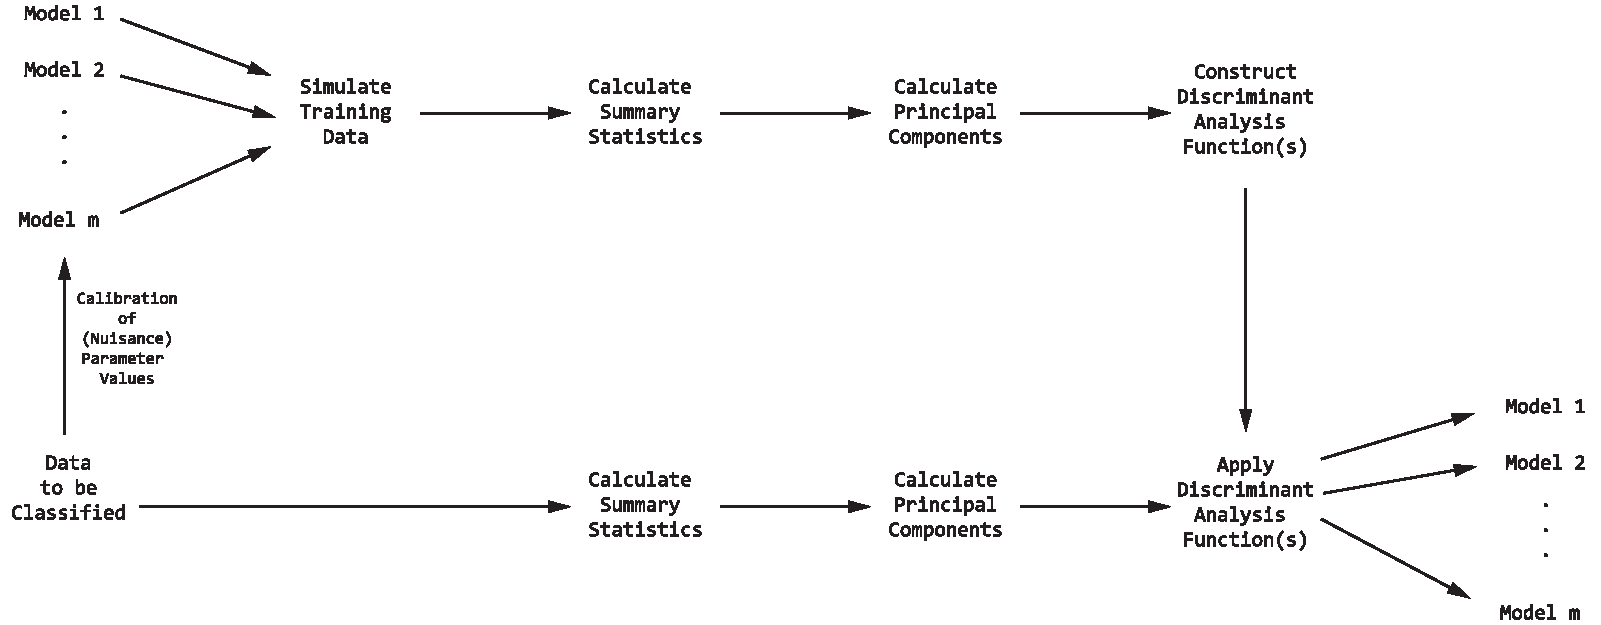
\includegraphics[scale=0.5]{figs/flowchart1.pdf}
        % \caption{default}
        % \label{fig:default}
    \end{center}
\end{figure}

Let $\targetData$ be the \textit{target} data, consisting of an ultrametric phylogeny with each of the tips associated with a geographic range (presence/absence over one or more areas) as well as with set of trait states.
Let $\modelCategories = \{\modelCategory{1}, \modelCategory{2}, ... \modelCategory{m}\}$ be a set of $k$ models that we are interested in studying.
Let $\summaryStatisticFunction(\cdot)$ be a function that takes a set of data returns a set of summary statistics.
Our analytical objective is, for each $\modelCategory{i}, \modelCategory{i} \in \modelCategories$, estimate the probability that it generated the target data $\targetData$, relative to all the other models in $\modelCategories$.
The operational procedure consists of the following steps:
\begin{enumerate}
    \item \textbf{Simulation of Training Data}: For each $\modelCategory{i}, \modelCategory{i} \in \modelCategories$, simulate $n$ replicates of data, $\trainingDataForModel{i}$. We label each replicate of this data with the name of the model that generated it (e.g., ``Model $i$''). The set of all data so generated constitutes the training data, $\trainingDataSet$.
    \item \textbf{Calculation of Summary Statistics}: Calculate summary statistics on the training data to yield, $\summaryStatisticFunction(\trainingDataSet)$, and summary statistics on the target data to yield $\summaryStatisticFunction(\targetData)$.
    \item \textbf{Classification of Target Data}: Construct a Discriminant Analysis (DA) function on principal components (PC) calculated on the training data set summary statistics, $\summaryStatisticFunction(\trainingDataSet)$; apply the discriminant analysis function to principal components calculated on the summary statistics of the target data, $\summaryStatisticFunction(\targetData)$.
\end{enumerate}

\subsection{Simulation of Training Data}

We use the program, ``\texttt{archipelago-simulate.py}'', to simulate the training data.

\end{document}
